\documentclass[11pt, oneside]{article}   	% use "amsart" instead of "article" for AMSLaTeX format
\usepackage{geometry}                		% See geometry.pdf to learn the layout options. There are lots.
\geometry{a4paper}                   		% ... or a4paper or a5paper or ... 
%\geometry{landscape}                		% Activate for for rotated page geometry
\usepackage[parfill]{parskip}    		% Activate to begin paragraphs with an empty line rather than an indent
\usepackage{graphicx}				% Use pdf, png, jpg, or eps§ with pdflatex; use eps in DVI mode
\usepackage{enumitem}
					% TeX will automatically convert eps --> pdf in pdflatex		
\usepackage{amssymb}
\usepackage{float}
\title{Masters' Project \\Michaelmas Progress Report}
\author{Patrick Lewis \\Queens' College}
\date{December 2015}							% Activate to display a given date or no date

\begin{document}
\maketitle
\begin{figure}[H]
    \centering
    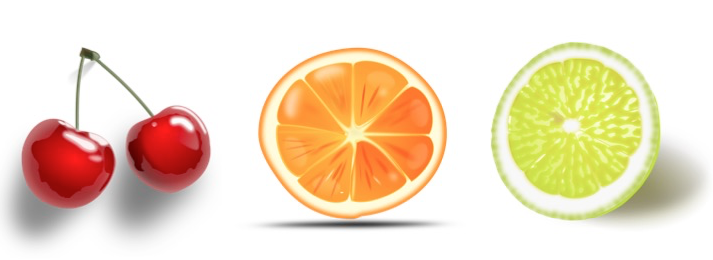
\includegraphics[scale=0.5]{TITLE.png}
\end{figure}
\section{Introduction}
\subsection{Modern Scientific Publishing}
With the widespread adoption of the internet in the late 1990's and 2000's, there were fundamental sweeping changes in the academic publishing landscape. The information revolution allowed publishers' costs to fall dramatically, and there was a mood shift in the academic sphere away from subscription based models, towards giving open and free access to some or all of journal article contents.

Simultaneously, university department websites began to post records of their recent publications for adverting and informational purposes, usually with hyperlinks to where the article could be fully accessed.

Publishers still protect journal article content and metadata, in some cases, aggressively, in order to protect their intellectual property. The data they hold on article publishing is immensively valuable and powerful, and as such, publishers are reluctant to give access to their massive metadata holdings. There is a well known saying in Data Science from Tim O'Reilly, ``The Guy with The Most Data Wins" \cite{HEWHOHASDATA}. As such, it is unlikely that academic publishing companies will release their data for analysis by the public in the near future.
\subsection{Motivation}
The publishing data, when collected and analysed using machine learning and big data techniques, can yield valuable insights into the direction of shifting academic focus, where world leading research is being carried out, and offers the possibility of procedural categorisation of research amongst many other possibilities. Large datasets are almost infinitely mine-able and interesting insights can be found `around every corner'. For an academic institution like the University of Cambridge, there are two main motivations for mining the data of the publishing landscape:
\begin{itemize}
\item{Purely Academic insights such as examination of the landscape's features , finding structural information and concealed relationships, in order to better understand how scientific information is spread throughout the world}
\item{Actionable insights, such as identifying where effective collaborations could be set up, prediction of where funding may been allocated, and identification of future areas of academic interests so that internal resources can be intelligently applied}
\end{itemize}
\subsection{Aims}
\label{sec:AIMS}
There are two main aims for the project, broken down below.
\begin{itemize}
\item{Data Collection - A scalable, legal and useful programmatic approach to scrape the online publishing landscape to collect as much useful data as possible.}
\item{Data Analysis - Once the data has been collected, Machine learning and statistical techniques should be applied to try and find insights within the data.}
\end{itemize}
The data analysis for such a large, rich dataset is a potentially never ending process. The strategy adopted is to focus on answering a smaller simpler research question first, building a structure to robustly test and answer that hypothesis and then to move on to new research questions.
As such, the first research question will be to build a system that can analyse the similarity between scientific authors. This will enable us to find where some authors are publishing qualitatively similar work to each other and to investigate the possibility of them collaborating. 
The framework upon which this research question is used immediately suggests new, similar questions that can be answered. As such, it will be a primary aim of the project to expose a useful framework for future probing to be facilitated (namely creating a chemistry semantic space where concepts can be quantitatively represented).

From a technical point of view, the aims of the project are as follows:
\begin{itemize}
\item{Provide documented, maintainable code}
\item{Provide a system that is as automated as possible}
\item{Provide a system that will automatically evolve and improve as time goes on}
\item{Provide a system that will not entropically lose data or suffer data degradation}
\item{Provide a system that produces interpretable, useful outputs}
\end{itemize}
The focus is on ensuring that the result of the project is a system that will continue to be useful after the programmer has left. This will require decent documentation discipline, and systems in place to manage crashing.
\section{First Steps}
\subsection{Generating XPaths}
The initial focus was on developing a strategy to scrape records off an unseen webpage.
Webpages are written in a tree-like structure using a markup language called HTML, (HyperText Markup Language). A very basic webpage is shown in Figure~\ref{fig:HTMLTREE}.When a webpage is accessed, the html code is sent over the internet to the user, and the browser e.g. Firefox, interprets it and displays the webpage in a human readable format. When scraping a page for information, the html code itself is scraped. The programmer must  write a program that accesses the useful parts of the webpage and stores the required information. 
\begin{figure}[H]
    \centering
    \textbf{HTML and XPaths}\par\medskip
    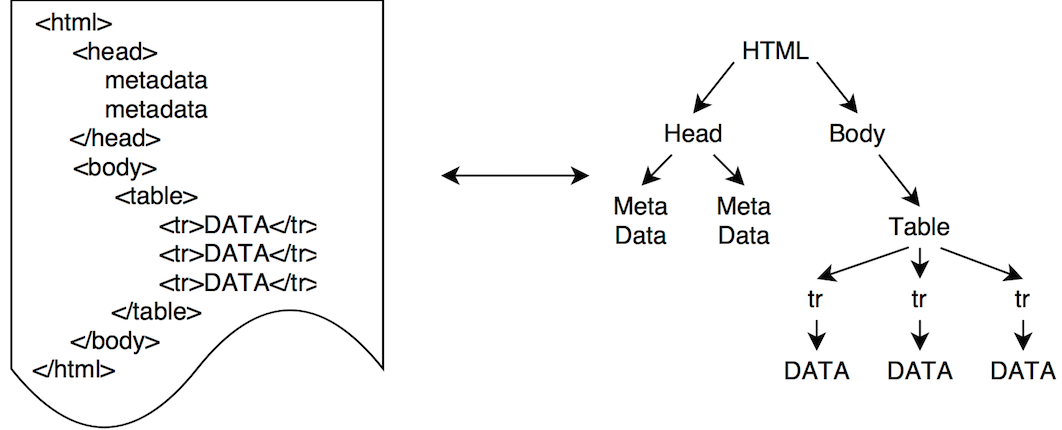
\includegraphics[scale=0.3]{HTMLTREE2.png}
    \caption{Tree representation of HTML code\label{fig:HTMLTREE}}
\end{figure}

In the above simplified example, it is shown that the html code represents a tree structure, and the useful data is at the bottom of the `body' branch. In order to store the DATA fields, the programmer must provide what is known as the XPath to that node in the tree. The XPath is just a set of directions that the program follows to find the data, and in the example above, the DATA fields are accessed via XPath:\begin{center} \texttt{//HTML/Body/Table/Tr/*}\end{center}
The XPath is a required part of any scraping strategy. The first problem with scraping potentially millions of webpages, is how the XPath (potentially very complicated, and certainly different for every single institution) can be generated. The initial approach was to write a tree analysis suite that would give the XPath of the most `probable' data entries. This worked by finding the most repeated substructure within the entire tree, and by using heuristics, parameters could be adjusted to automatically generate the XPath to the useful data with decent efficiency. 
The core of the algorithm is shown below: 
\begin{sloppypar}
\begin{enumerate}
\item \texttt{Start at trunk of tree}
\item \texttt{Count the number of descendants of each child of the current node}
\item 
\begin{enumerate}
\item \texttt{Check if all child notes are all within a threshold of similarity to each other}
\item \texttt{Check there are more than a required threshold number of child nodes}
\item \texttt{Check the average similarity between child nodes is above a certain threshold}
\item \texttt{Check that the proportion of child nodes that are considered `similar' is above a certain threshold}
\end{enumerate}
\item \texttt{If all of (a)-(d) are true, this node contains the required data and the XPath has been found. Otherwise, move down to the child node with the greatest number of descendants and return to step 2}
\end{enumerate}
\end{sloppypar}
The thresholds mentioned in steps 3.(a)-(d) are adjustable parameters set at reasonable values. This approach was successful for webpages with very large numbers of records on them, as the algorithm searches for the largest, most frequently repeating structural unit in the tree. If there are not vast numbers of records on the page, the method can fail.
As such, this strategy is not flexible enough for the required purposes. Despite this it is still useful and still the quickest automated way to generate XPaths for webpages with many hundreds of records on them. A different strategy has been been adopted, which is discussed in detail in section \ref{sec:COLLECTIONSTRATEGY}.
\subsection{CAMSIM and BATHSIM Mini Projects}
\label{sec:CAMSIM}
A significant part of the first few weeks of the project were dedicated to selecting and learning the appropriate technologies to achieve the goal. The CAMSIM and BATHSIM projects were small proof of concept projects to explore how the different technologies work together, and to prototype a system architecture.
The techologies used are:
\begin{enumerate}
\item Python 2.7.10 programming language. A modern and flexible interpreted programming language widely adopted by the scientific community, Python 2 has many useful libraries available, optimised for use.
\item MongDB database - MongoDB is becoming one of the most popular databases for data intentsive applications \cite{BIGMONGO}. MongDB is a schema-less noSQL database - it records objects as individual, unstructured `documents' rather than as rows in tables. This is well suited to the task as complete data is not always available during large scraping operations. There are also well supported python drivers for MongoDB. 
\item Anaconda Environment - Anaconda is a python distribution/virtual environment, allowing quick use of external python packages, and fast generation of distributions to deploy on new machines.
\item Scrapy Scraping suite - A well supported end to end scraping framework for Python, allowing fast, scalable web scraping. 
\item Gensim - A Natural Language Processing and Machine Learning suite for Python. Their libraries are C optimised and widely used and verified.
\end{enumerate}

\begin{figure}
    \centering
    \textbf{CAMSIM and BATHSIM Architecture}\par\medskip
    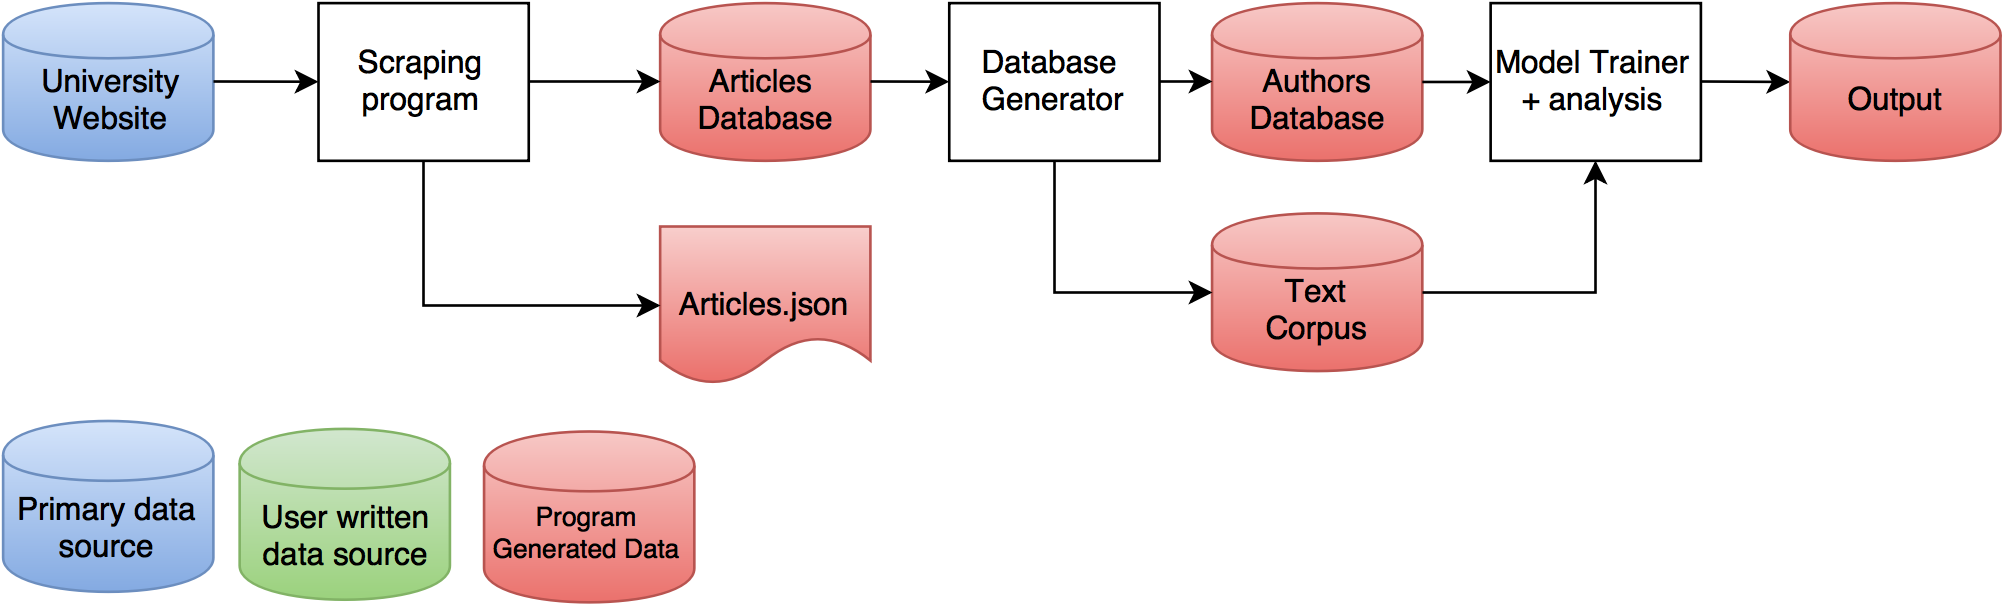
\includegraphics[scale=0.23]{CAMSIM.png}
    \caption{Flow Chart Diagam representing CAMSIM and BATHSIM structure \label{fig:CAMSIM}}
\end{figure}

BATHSIM and CAMSIM projects use all of the above technologies with an architecture shown in Figure ~\ref{fig:CAMSIM}. The programatic flow is represented above. BATHSIM and CAMSIM have the same structure, and the only difference is the source data for CAMSIM is provided by University of Chemistry Department at \texttt{ http://www.ch.cam.ac.uk/publications} whereas BATHSIM's source is the data provided by the Bath University Chemistry department, at \texttt{http://opus.bath.ac.uk/view/divisions/dept=5Fchem.html}. A custom written scraping program collects the data which is placed into a database and exported as a human readable .JSON text file. A second program then creates databases of individual authors and a corpus of all the collected titles and abstracts (explained further in section \ref{sec:DATAPROC}). As discussed in the section \ref{sec:ANALYSIS}, this corpus is used to train a Word2Vec style model that generates a vector representation of an author's published work. The dot product cosines between authors' vectors are computed and outputted as a measure of their similarity.
\section{Collection Strategy}
\label{sec:COLLECTIONSTRATEGY}
The main problem encountered so far is how to scrape large numbers of websites for records without writing tailored time consuming scraping scripts and finding XPaths for every website visited, (approach used in CAMSIM and BATHSIM). The possible solution is using `regular expression' pattern matching techniques on DOIs. DOIs are explained in detail in section \ref{sec:DOI}. The proposed collection strategy, which is nearly complete, is then described in section \ref{sec:CHERRY}.
\subsection{DOI}
\label{sec:DOI}
DOIs (document object identifiers) are identifier strings used access journal articles. DOIs can issued by a number of accredited issuing bodies, although the vast majority of scientific articles are issued by CrossRef, a not-for-profit body comprised from Publishers International Linking Association (PILA), a loose association of many academic publishers \cite{CROSSREF}. A DOI is usually included in a citation or record, and by pre-pending a DOI string with the url stub \begin{verbatim} http://dx.doi.org/ \end{verbatim}, DOI.org will redirect the request to the desired academic journal entry on the publisher's website. All articles published by large established publishers since the adoption of the DOI system will have a DOI registered against them.

DOIs have a somewhat loose structure, and the `anatomy' of a DOI is shown in figure \ref{fig:DOI}.

\begin{figure}[H]
    \centering
    \textbf{Anatomy of a DOI}\par\medskip
    \includegraphics[scale=0.15]{DOI2.png}
    \caption{Doi structure. The structure consists of a numeric prefix (X and Y must be integers) and alphanumeric suffix (Z can be any UTF-8 encoded Character) \label{fig:DOI}}
\end{figure}
DOIs consist of 2 sections, the prefix and suffix. The prefix is subdivided into a `Directory Indicator' (always integer `10') separated from a `Registrant Code' assigned by the issuing body. Registrant codes are numeric and can be of any length, however they are almost invariably 4 integers long. Registrant codes can have further subdivisions separated by full stops. The suffix is provided by the registrant themselves. It can have any form as long as it is encodable by UTF-8. The DOI specification somewhat ambiguous as there is no vigorous way to terminate a DOI, and on a webpage, the end of a DOI suffix must be interpreted from the context. This provides some scraping difficulties, but can be overcome with careful consideration of outlier cases.
\subsection{Cherry Data Collection Program}
\label{sec:CHERRY}
DOIs can be recognised programmatically from HTML source code through the use of regular expression pattern matching techniques. This suggests a way to collect article data without knowledge of the XPath. 
The new strategy for creating a widespread scraping with well structured output data is summarised below.
\begin{sloppypar}
\begin{enumerate}
\item \texttt{Download page source of university website}
\item \texttt{Use pattern matcher to extract DOIs from the source HTML code}
\item \texttt{Verify scraped DOIs by using CROSSREF API service}
\item \texttt{Deposit valid DOIs in DOI Database}
\item \texttt{Use collected DOIs and DOI.org re-routing service  to access publisher webpages for articles}
\item \texttt{Extract useful, freely available article data: Title, Authors, Date, Abstract, Affiliations}
\item \texttt{Store these full records in a database, for use in data analytics}
\end{enumerate}
\end{sloppypar}
This process allows widespread scraping as XPaths are only required for the publisher webpages, rather than the university websites. There are much fewer publisher website formats than potentially infinite formats for university websites, and a conversion rate of \textgreater 90\% has already been achieved on a sample dataset of DOIs to full records, from only $\sim$20 publisher websites XPath sets. 
The algorithm above is to be implemented by the system architecture shown in figure \ref{fig:CHERRY}.

\begin{figure}[H]
    \centering
    \textbf{Cherry Program Architecture}\par\medskip
    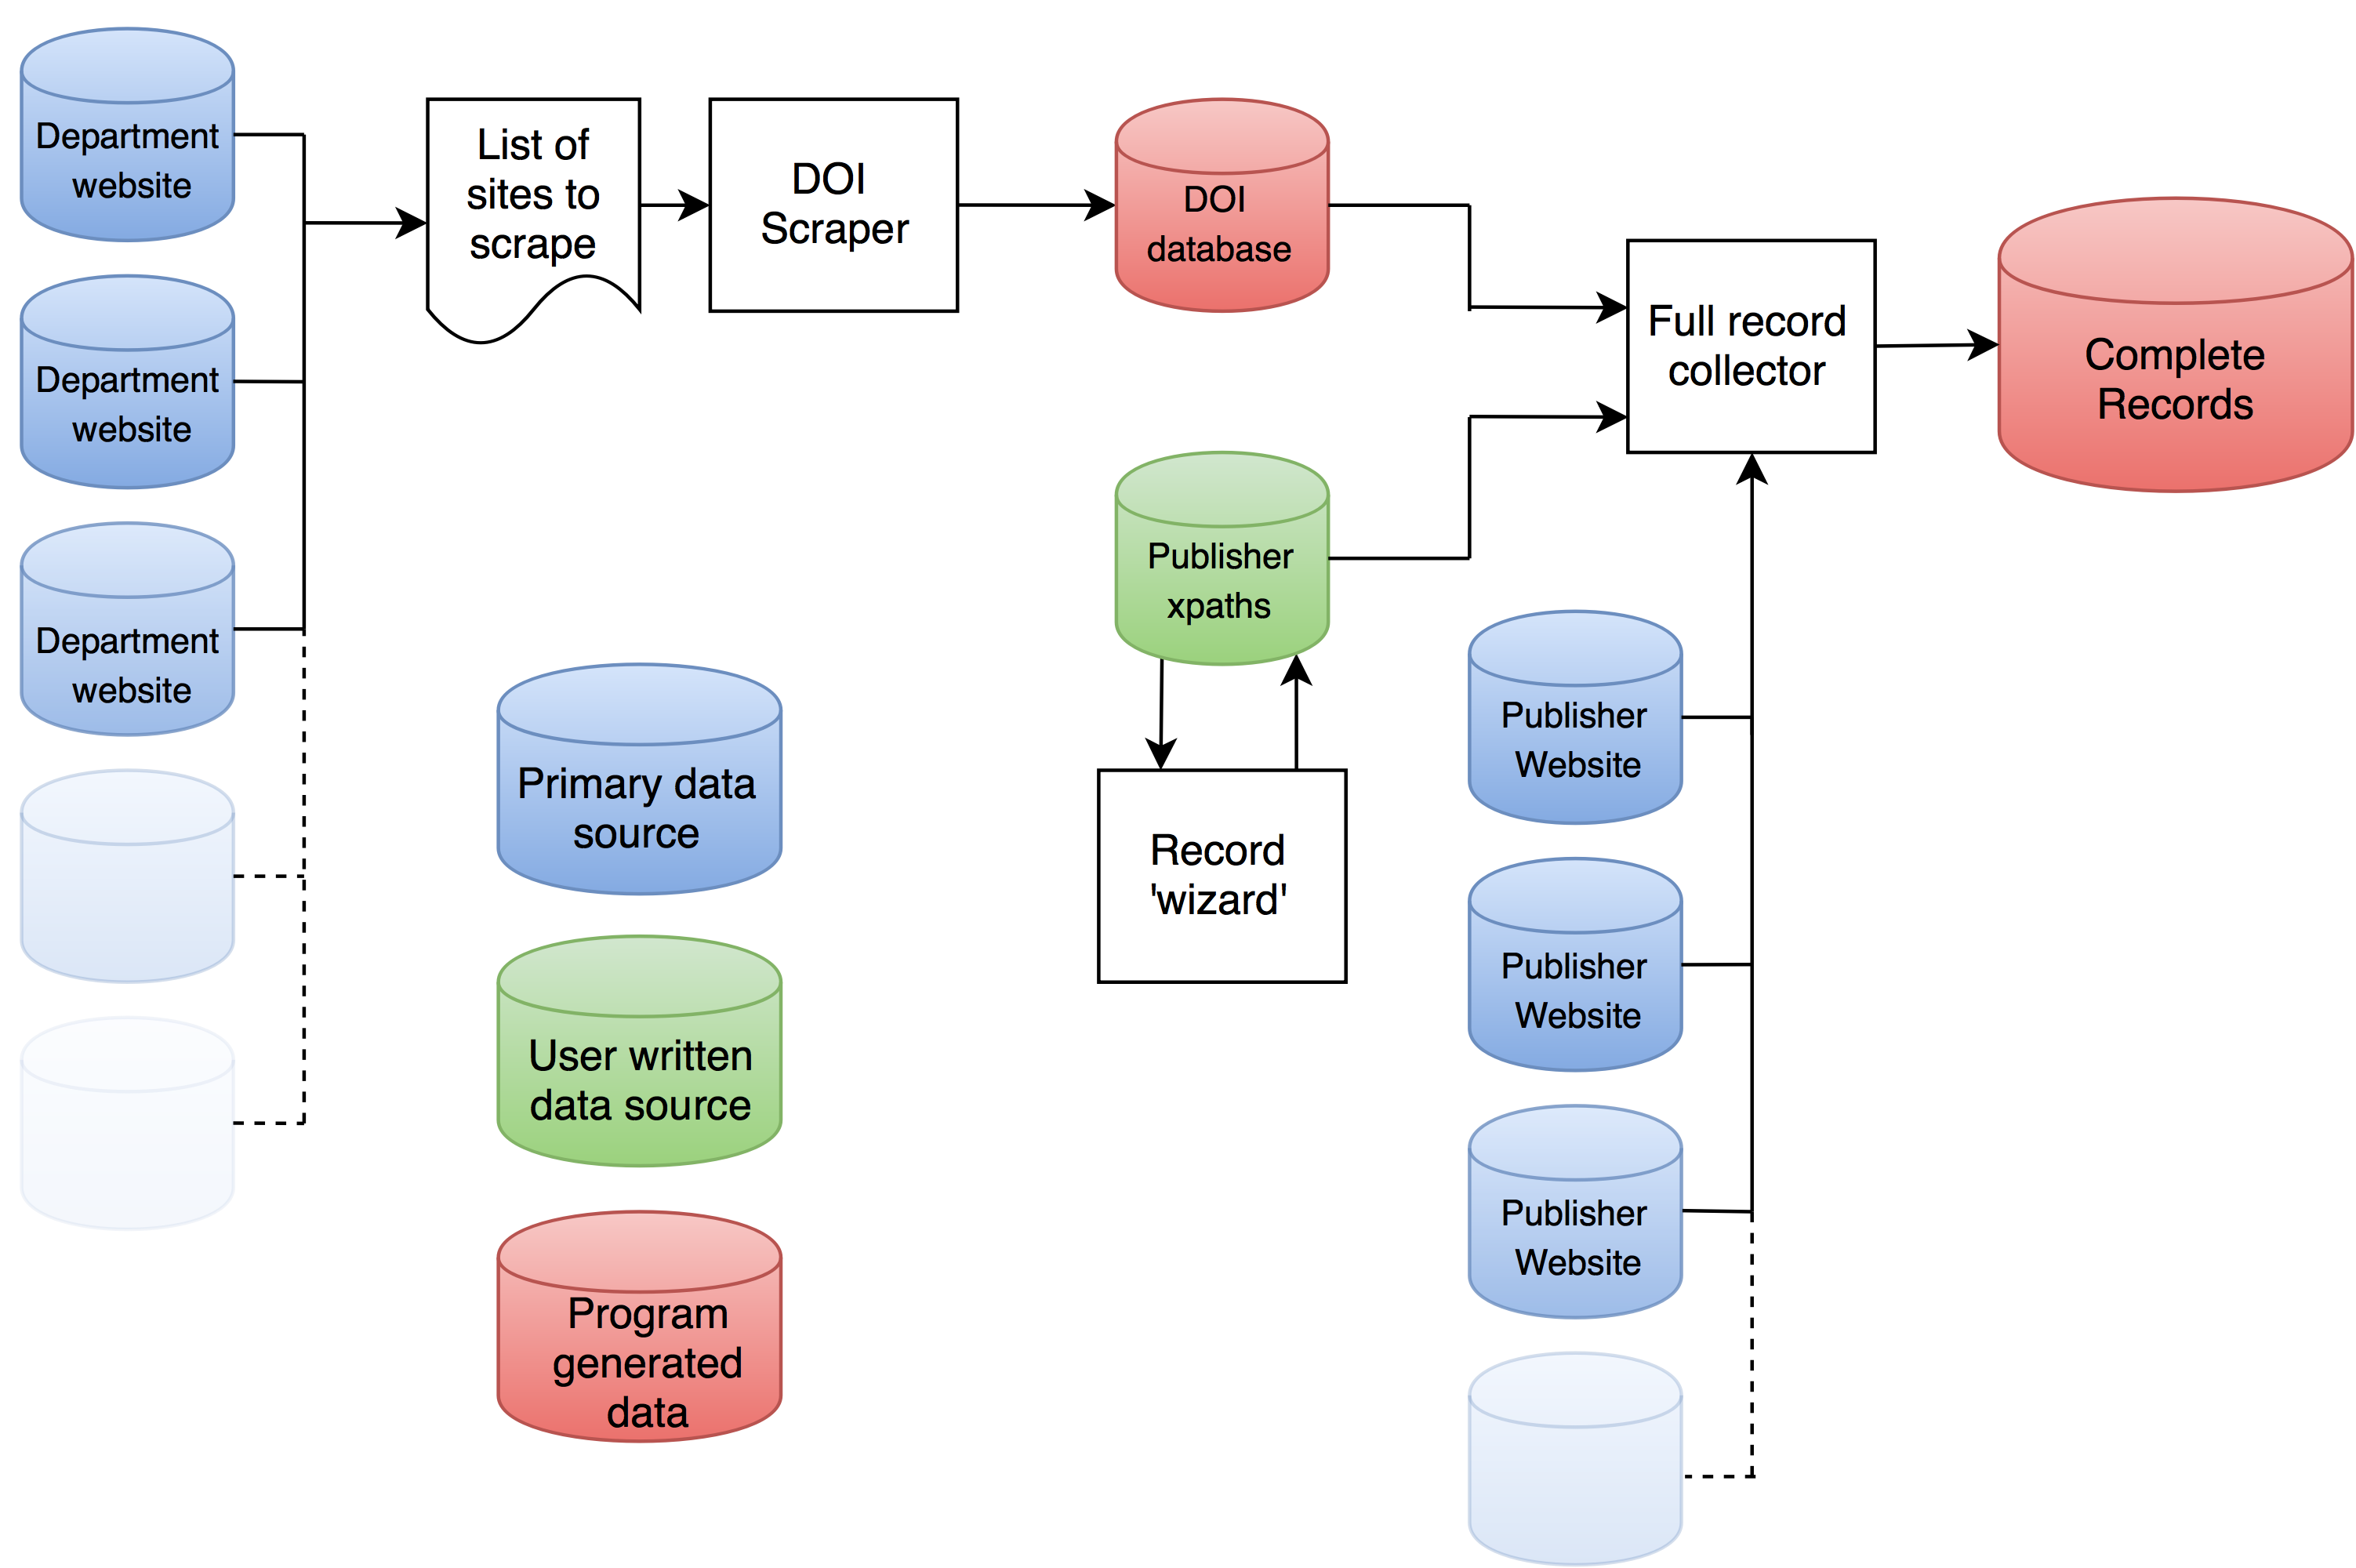
\includegraphics[scale=0.15]{CHERRY.png}
    \caption{Flow Chart Diagram representing data collection strategy structure \label{fig:CHERRY}}
\end{figure}
The system has been named Cherry, as the process is reminiscent of picking cherries from an `html tree', and then eating them. The naming convention of fruit runs through into the next sections. 
The Cherry data collection system is 90\% complete at time of writing, with the programs referred to in \ref{fig:CHERRY} as `DOI SCRAPER' being complete and `Full Record Collector' being put through thorough testing. The `Publisher XPaths' database is an ongoing project, and can never be `complete'. It is the only brittle part of the program and will necessarily need to added to in order to incorporate more publishers and updated when publisher websites change. 
`Record Wizard' is a proposed program to help write the XPaths and the small normalisation processes required to collect full records for a given publisher website. As an auxiliary program not vital to the system to run, it is of lower priority and will be implemented when the system is up and running.
\section{Analysis}
\label{sec:ANALYSIS}
\subsection{Algorithm}
The core aim is to be able to represent research interests quantitatively so that programatic comparisons and analysis can be facilitated. The algorithm that will be used for this purpose is a recently published Natural Language Processing deep learning techique known as Word2Vec\cite{WORD2VEC}\cite{PHRASE2VEC}. The Word2Vec algorithm is a based off  `continuous Skip-Gram' and `Continuous Bag of Words' architectures. These two learning algorithms are highly optimised, research level Natural language processing algorithms. Word2Vec, after training, takes in individual words and outputs vector representations of those words. The `Continuous Bag of Words' (henceforth CBOW) learns by attempting to predict the current word based on the word's context (specifically the 2 words preceding and the 2 words following) during training and the `skip-gram' model learns by attempting to predict the surrounding words given the current word. They could be considered as 1mirror image' techniques of each other.

As mentioned above, the Word2Vec algorithm, once trained on a corpus of many sentences, takes in individual words and converts them into n-dimensional vectors in a language space (n is a user specified value). These vectors encapsulate the syntactic and semantic meaning behind the words. The vectors can be manipulated in surprisingly elaborate ways, and the model can be evaluated by performing vector additions to represent concepts (more on this below). An example is shown in figure \ref{fig:KINGQUEEN}
\begin{figure}[H]
    \centering
    \textbf{Word Vector Relationships}\par\medskip
    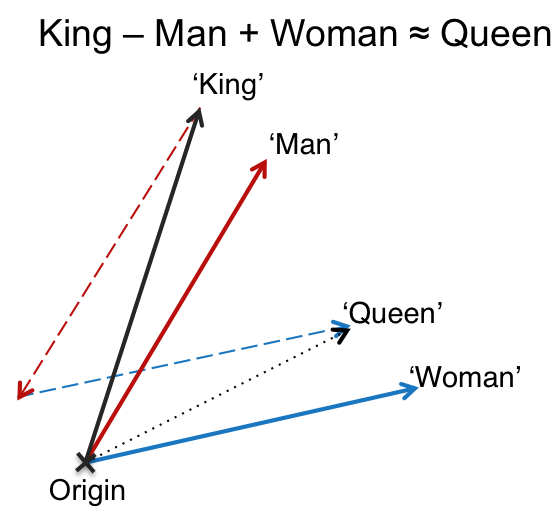
\includegraphics[scale=0.7]{KINGQUEEN.png}
    \caption{Schematic Representation of how concepts can be represented in word vector space. Word2Vec is able to replicate this behaviour. The vector found by vec(`King')-vec(`Man')+vec(`Woman') is approximately equal to vec(`Queen'). The model has been tested on thousands of similar examples\cite{WORD2VEC}  \label{fig:KINGQUEEN}}
\end{figure}
  

 The CBOW and Skipgram algorithms have different strengths but vigorous testing of which will be the best choice for the task cannot be completed until a large set of training and testing data have been amassed. The CBOW appears to be better for syntactic relationships, and Skipgram better for semantic relationships\cite{WORD2VEC}:
\begin{itemize}
\item Syntactic relationship: \emph{good} is to \emph{better} as \emph{rough} is to ... (expected answer: `rougher')  \cite{LINGUISTICREG}
\item Semantic relationship: \emph{clothing} is to \emph{shirt} as \emph{dish} is to ... (expected answer: some specific type of dish, e.g.`bowl')  \cite{LINGUISTICREG}
\end{itemize}
The purpose of the task is to compare semantic chemical concepts, so it may prove that skipgram is a better fit for the purposes, however it will be an interesting question to compare outputs from both models.

The models themselves learn with the following basic method. Sentences of words are assumed to contain words that are semantically and syntactically related. If two words appear in the same sentence, they can assumed to be in some way `similar'. Word vectors are randomly initialised, and then iteratively optimised, so that weights of word-word connections in the internal network are strengthened if that word pair appear often in sentences together. The procedure is somewhat similar to Neural Network techniques, with only an input and output layer (no non-linear hidden layers). The training complexity is greatly improved over Neural Network techniques.\cite{WORD2VEC}.

\subsection{Data processing}
\label{sec:DATAPROC}
The `Cherry' database generated from the process described in section \ref{sec:CHERRY} contains much free text (the titles and abstracts of the articles). These are already composed of concept linked sentences and can easily be fed in as training data into the Word2Vec algorithms. The more data used in training, the better the model will be. This requires a database with a great many records\cite{HEWHOHASDATA}\cite{WORD2VEC}. 

A training corpus is prepared from the `Cherry' database in a processing pipeline described in figure \ref{fig:CORPUSGEN}.
\begin{figure}[H]
    \centering
    \textbf{Training Corpus}\par\medskip
    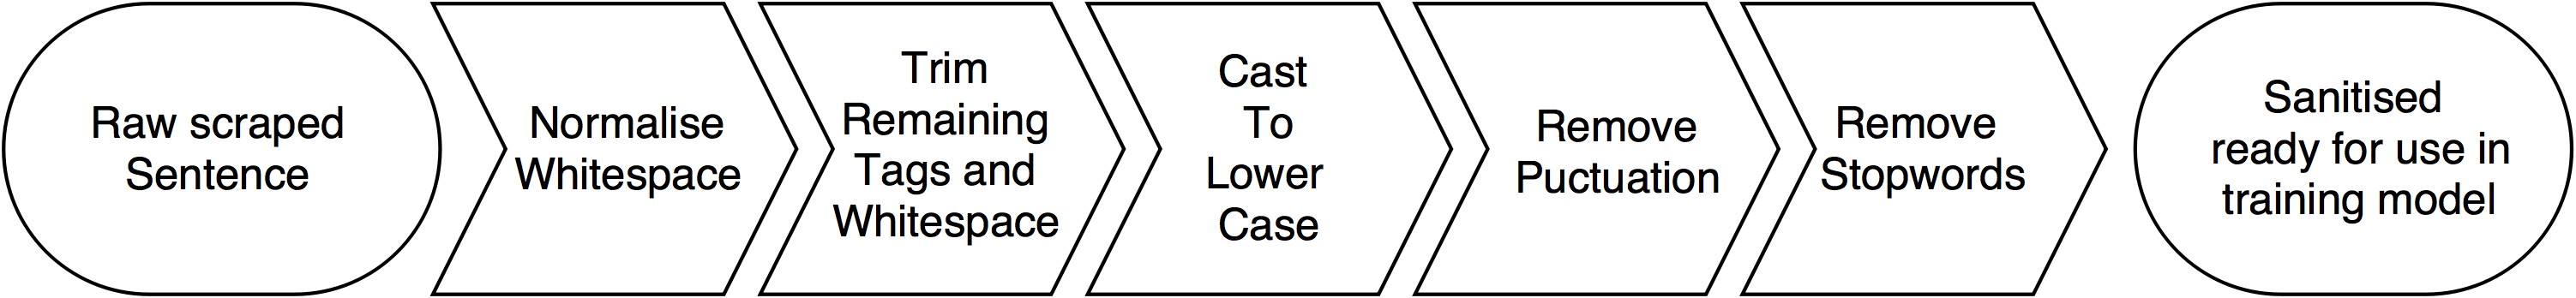
\includegraphics[scale=0.14]{CORPUSGEN.png}
    \caption{figure showing how data is sanitised and aggregated into the training corpus for training the Word2Vec model \label{fig:CORPUSGEN}}
\end{figure}
The training corpus is then used to train a Word2Vec model, which in turn can be used to generate vectors to represent e.g. articles, concepts and author research interests (this list is not exhaustive). The analysis suite that will perform these tasks is summarised in the architecture diagram in figure \ref{fig:ORANGELEMON}.
\begin{figure}[H]
    \centering
    \textbf{Oranges and Lemons Program Architecture}\par\medskip
    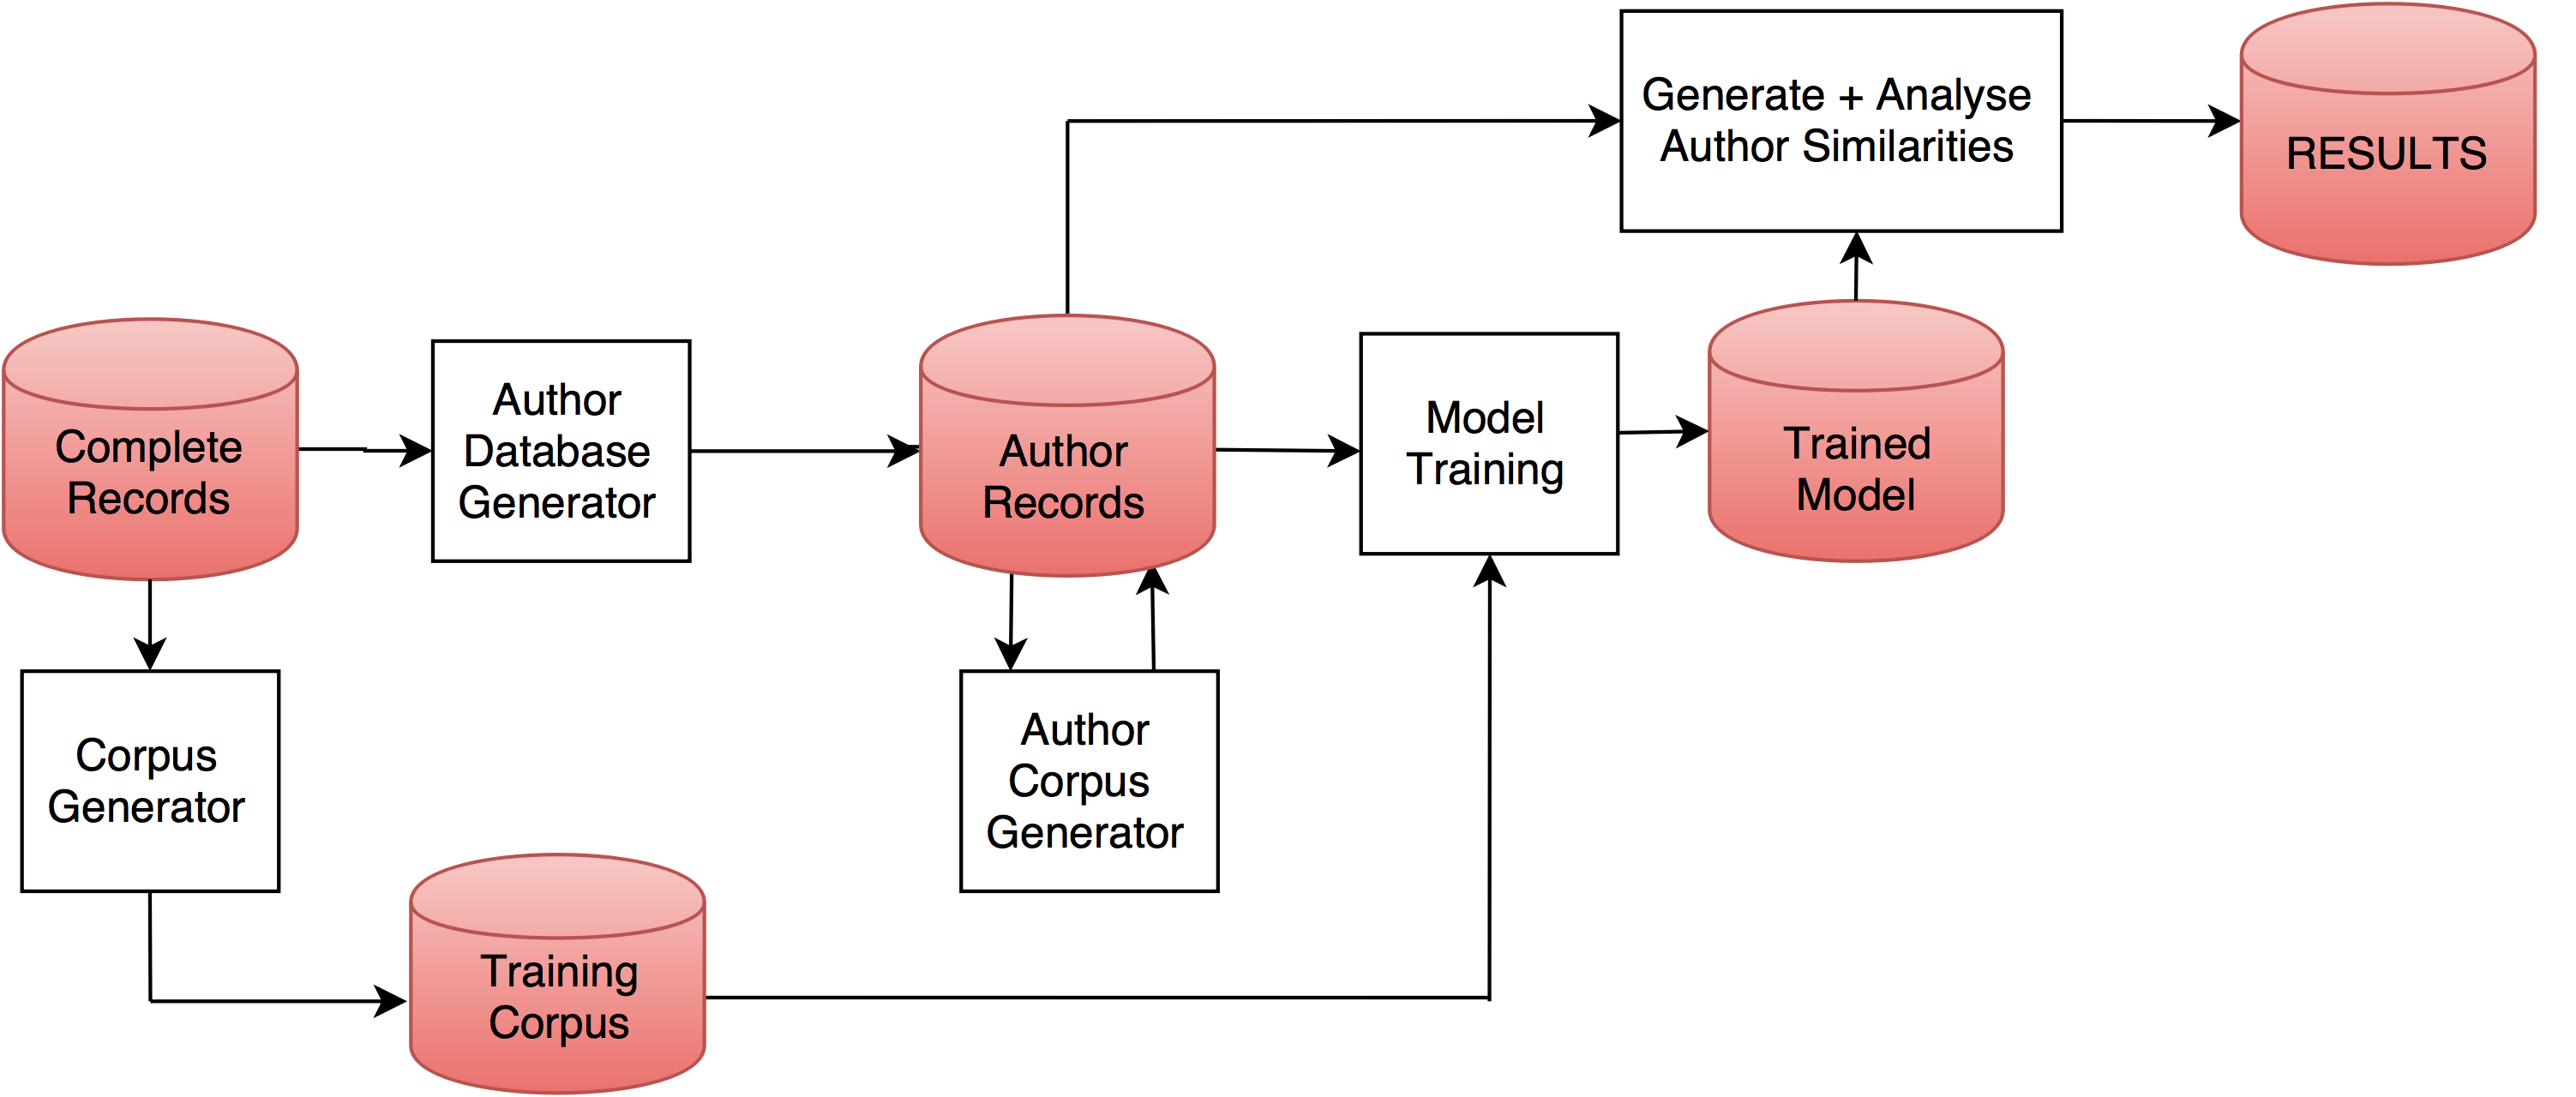
\includegraphics[scale=0.14]{ORANGESLEMONS.png}
    \caption{Flow Chart Diagram representing data analysis, training and transformation programmatic structure \label{fig:ORANGELEMON}}
\end{figure}
Figure \ref{fig:ORANGELEMON} includes the necessary programing structure to fulfil the analysis in described in section \ref{sec:LEMON}. The naming convention of fruit was continued from the collection suite described in \ref{sec:CHERRY}. `Oranges' is the name given to the corpus generation and model training processes, whereas `Lemons' is the process required to fulfil the analysis in section \ref{sec:LEMON}. Names for analyses outlined in sections \ref{sec:KMEANS}, \ref{sec:TIMETRACK} and \ref{sec:NETVIS} will be assigned when the tasks themselves are addressed.
\subsubsection{Author similarity pairs}
\label{sec:LEMON}
By collecting together articles associated with an author and sanitising the titles and abstracts with the same process descibed in figure \ref{fig:CORPUSGEN}, we can create a set of words that represent the author's research interests.Each of these words will each have a vector associated with them, $\mathbf{w_i}$ extracted from the trained Word2Vec model. These can be aggregated to form an average vector of the author's research interests, $\mathbf{a}$:
$$\mathbf{a} =  \frac{1}{N}\displaystyle\sum_{i=1}^{N} \mathbf{w_i} \mbox{ where N is number of author representation words}$$
The similarity between two authors $\alpha$ and $\beta$ can measured by finding the cosine similarity between their vectors:
$$\mathbf{a^{(\alpha)}}.\mathbf{a^{(\beta)}}=\displaystyle\sum_{\gamma=1}^{D} \nu^{(\alpha)}_{\gamma}\nu^{(\beta)}_{\gamma} = |\mathbf{a^{(\alpha)}}||\mathbf{a^{(\beta)}}|cos(\theta) $$
where the dimensionality of the vector space is $D$ and the components of a vector $\mathbf{a}$ are $(\nu_1,\nu_2...\nu_D)^T$. The cosine similarity $cos(\theta)$ is easily computable:
$$cos(\theta)= \frac{\displaystyle\sum_{\gamma=1}^{D} \nu^{(\alpha)}_{\gamma}\nu^{(\beta)}_{\gamma}}{\left(\displaystyle\sum_{\gamma=1}^{D} (\nu^{(\alpha)}_{\gamma})^2\right)^{1/D} \left(\displaystyle\sum_{\gamma=1}^{D} (\nu^{(\beta)}_{\gamma})^2\right)^{1/D}}$$
which can be well optimised in coding using standard computational libraries.
For an author pair, a cosine similarity of $\approx$1 can be interpreted as the two authors having very similar research interests. These high cosine similarities may reveal interesting links between authors currently separated from each other.

This analysis can be achieved programmatically by the structure outlined in figure \ref{fig:ORANGELEMON}. The `Lemon' analysis process generates a database of authors from the Cherry database described in section \ref{sec:COLLECTIONSTRATEGY} and creates a `mini corpus' of representative published words for each author in the database. The analysis suite then computes author vectors and pairwise generates cosine similarities between authors. The process of creating author pairs is not exhaustive as the pairwise comparison complexity will scale with O$(n^2)$. For a set of 1000 authors, to fully explore similarities will require $n(n-1)/2 \approx 500,000$ cosines to be computed. For a very large database, it may be impractical to generate all similarity pairs. Batch processing and intelligent storage of previously computed pairs may however enable thorough searching of the space. The programmatic mechanics of `Lemons` have been written and a rudimentary form was used in the proof of concepts CAMSIM and BATHSIM (see section \ref{sec:CAMSIM}). The models used for vector generation did not have sufficient training data to output useful results. This will change with the completion of `Cherry' when much more data can be collected. 
\subsubsection{K-means clustering of research landscapes}
\label{sec:KMEANS}
K-Means clustering is a categorisation technique in machine learning where k cluster centres are optimised to have least distance from a set of data points. After some dimensional reduction of a set of research interest vectors produced from the `Cherry' database, k-means clustering could be used to identify research clusters. When the means have been found, new (unseen) articles could be assigned to a topic based on the proximity to the closest cluster centre. 
\subsubsection{Tracking of Research interests with time resolution}
By calculating two sets of k-means cluster centres from two sets of vectors from articles published from two different years, and by tracking how the cluster centres have moved over time, it may be possible to infer how the focus of research has changed over time. As an extension, if the data is of high enough quality, it may be possible to extrapolate where the clusters may move to in the future. 
\label{sec:TIMETRACK}
\subsection{Network visualisation}
Using tools such as Gephi, pairwise author similarity should be able to be visualised as a network graph. This may elucidate non-obvious connections between authors and departments.  
\label{sec:NETVIS}
\section{Next Steps}
The next steps suggest themselves naturally. The immediate priority is to finish the `Cherry' framework and set to work giving it websites to digest. After that has been finished, the focus shifts into analysis, and gluing existing scripts together to get the `Oranges' and `Lemons' programs running. 
The analyses suggested in \ref{sec:KMEANS} \ref{sec:TIMETRACK} and \ref{sec:NETVIS} are stretch goals of the project, and will probably fall outside the time frame. There is much potential of the method laid out in this document, but so little time to explore it. 
The portability, distributivity and usability goals alluded to in section \ref{sec:AIMS} may have to be completed after the final report submission date, as the final report will require findings, and due to the time constraints, this must be the priority. 
\label{sec:NEXTSTEPS}
\begin{thebibliography}{9}
\bibitem{HEWHOHASDATA} O'Reilly (2012) \emph{Tim O'Reilly interviewed by Forbes Editor Jon Bruner} Available at: \begin{verbatim}https://www.youtube.com/watch?v=wNLhFi3XhIE \end{verbatim} (accessed 24 November 2015)
\bibitem{BIGMONGO} 
\emph{JasperSoft Publishes Second Big Data Index} (2012) Available at
\begin{verbatim} http://www.jaspersoft.com/press/jaspersoft-publishes-second-big-data-index \end{verbatim} (accessed: 27 November 2015)
\bibitem{CROSSREF}
\emph{The Formation of CrossRef: A Short History} (2009) Available at: 
\begin{verbatim}http://www.crossref.org/08downloads/CrossRef10Years.pdf\end{verbatim} (accessed 25 November 2015)
\bibitem{DOIHANDBOOK}
\emph{The DOI Handbook - Numbering} (2014) Available at: \begin{verbatim}https://www.doi.org/doi_handbook/2_Numbering.html#2.2.2\end{verbatim} (accessed 25 November 2015) 
\bibitem{WORD2VEC}
T Mikolov, K Chen, G Corrado, J Dean.(2013) \emph{Efficient estimation of word representations in vector space. } ICLR Workshop, Available at: \begin{verbatim}http://arxiv.org/pdf/1301.3781v3.pdf\end{verbatim} (accessed 25 November 2015) 
\bibitem{PHRASE2VEC}
T Mikolov, I Sutskever, K Chen, G Corrado, J Dean .(2013) \emph{Distributed Representations of Words and Phrases and their Compositionality} NIPS,  Available at: \begin{verbatim}http://papers.nips.cc/paper/5021-distributed-representations-of-words-and-phrases-and-their-compositionality.pdf\end{verbatim} (accessed 25 November 2015) 
\bibitem{LINGUISTICREG}
T. Mikolov, W.T. Yih, G. Zweig.(2013) \emph{Linguistic Regularities in Continuous Space Word Representations} NAACL HLT, Available at \begin{verbatim}http://www.aclweb.org/anthology/N13-1090\end{verbatim} (accessed 25 November 2015) 

\end{thebibliography}
\end{document}  